%% 
%%	This is file 'beamer_sample.tex'
%%	according to an MPIDR's PowerPoint template (?)
%%	
%%	by Eric Naujoks
%%
%%	Problems, bugs and comments to 
%%	naujoks@demogr.mpg.de
%%

%%%%%%%%%%%%%%%%%%%%%%%%%%%%%%%%%%
%%	Praelegomena								%%
%%%%%%%%%%%%%%%%%%%%%%%%%%%%%%%%%%
%%	- Make sure that you use utf8-encoding for all your .tex-files!!! (TeXnicCenter since version 2.0)
%%	- TeXnicCenter update: MPIDR intranet > Hard- & Sortfware > Software > Script and text editors > TeXnicCenter

\documentclass[20pt,usenames,dvipsnames]{beamer}

\usepackage[ngerman,english]{babel}
\usepackage{tikz}
\usepackage[normalem]{ulem}
\geometry{paperwidth=10in, paperheight=7.5in}
\usepackage{animate}

\usepackage[utf8]{inputenc}

\usepackage[mpidr]{./mpidr/beamerthemeMPIDR}
%\usefonttheme{serif}
%\newcolumntype{C}[1]{>{\centering\let\newline\\\arraybackslash\hspace{0pt}}m{#1}}
%\newcommand*{\QEDA}{\hfill\ensuremath{\blacksquare}}
%% Declaring title and author
%	the institute's logo
%\renewcommand{\mylogo}{\includegraphics[width=4.7in]{mpidr_logo_colour_en}}
\usepackage{color}
\definecolor{mygray}{rgb}{0.8,0.8,0.8}
\definecolor{yellow}{rgb}{1,1,0}

\defbeamertemplate{description item}{align left}{\insertdescriptionitem\hfill}
%%	should be the very last package to be loaded
\usepackage{hyperref}

%%%%%%%%%%%%%%%%%%%%%%%%%%%%%%%%%%
%%	Beginning of the document		%%
%%%%%%%%%%%%%%%%%%%%%%%%%%%%%%%%%%
\begin{document}

%%	titlepage - fixed frame:
%%	========================

% \begin{frame}
% 	\titlepage
% \end{frame}
\begin{frame}[plain]
	%\titlepage
	\vspace{-3cm}
 \centerline{\includegraphics[scale=.165]{beamerstrip3.png}}

	
	\huge
	\vspace{1em}
	
	Alignment, clocking, and macro patterns of episodes in the life course\\
	\vspace{1em}
	\large 
	Tim Riffe 
\end{frame}
%-------------------

% motivation:
% 1) late-life sequence analysis ending in death (pattern detection)
% 2) matrix expression for average number of episodes (tenure statistics)
\begin{frame}[plain]
\Large
\centering
 2 motivating observations:\vspace{2em}
 \begin{enumerate}[<+->]
 \item sequence analysis of trajectories ending in death \only<3-4>{\textcolor{red}{(pattern detection)}} \only<4>{(Y. Hu)}
 \item matrix expression for average episode count \only<3-4>{\textcolor{red}{(tenure statistics)}} \only<4>{(C. Dudel)}
 \end{enumerate}
 % get screenshot from June, also paper from Dudel in email.
\end{frame}
%

\begin{frame}[plain]
\Large
\centering
 2 motivating questions:\vspace{2em}
 \begin{enumerate}
 \item would different patterns emerge if trajectories were aligned on moment of death rather than age?
 \item what is the age pattern of average episode duration?
 \end{enumerate}
 % get screenshot from June, also paper from Dudel in email.
\end{frame}
%

\begin{frame}[plain]
\Large
\centering
 2 \emph{procedural} solutions:\vspace{2em}
 \begin{enumerate}
 \item restructure wrt state transitions: \only<2>{\textcolor{red}{alignment}}
 \item flexible episode recording: \only<2>{\textcolor{red}{clocking}}
 \end{enumerate}
 % get screenshot from June, also paper from Dudel in email.
\end{frame}
%

\begin{frame}[plain]
\Large
\begin{center}
An illustration
\pause
\begin{itemize}[<+->]
  \item Take transition matrix from \normalsize{Dudel \& Myrskl\"a (2017)}.
  \item Simulate 10k trajectories using \texttt{rmarkovchain()} in \texttt{markovchain}
  package \normalsize{(Spedicato, 2017)}.
  \item Demonstrate concepts of \textcolor{red}{alignment} and \textcolor{red}{clocks}
  \item Generate (stationary) novel macro patterns
\end{itemize}
\end{center}
\end{frame}

\begin{frame}[plain]
\Large
\begin{center}
Clock measures
\vspace{1em}
\begin{overlayarea}{\textwidth}{.4\textheight}
\only<1>{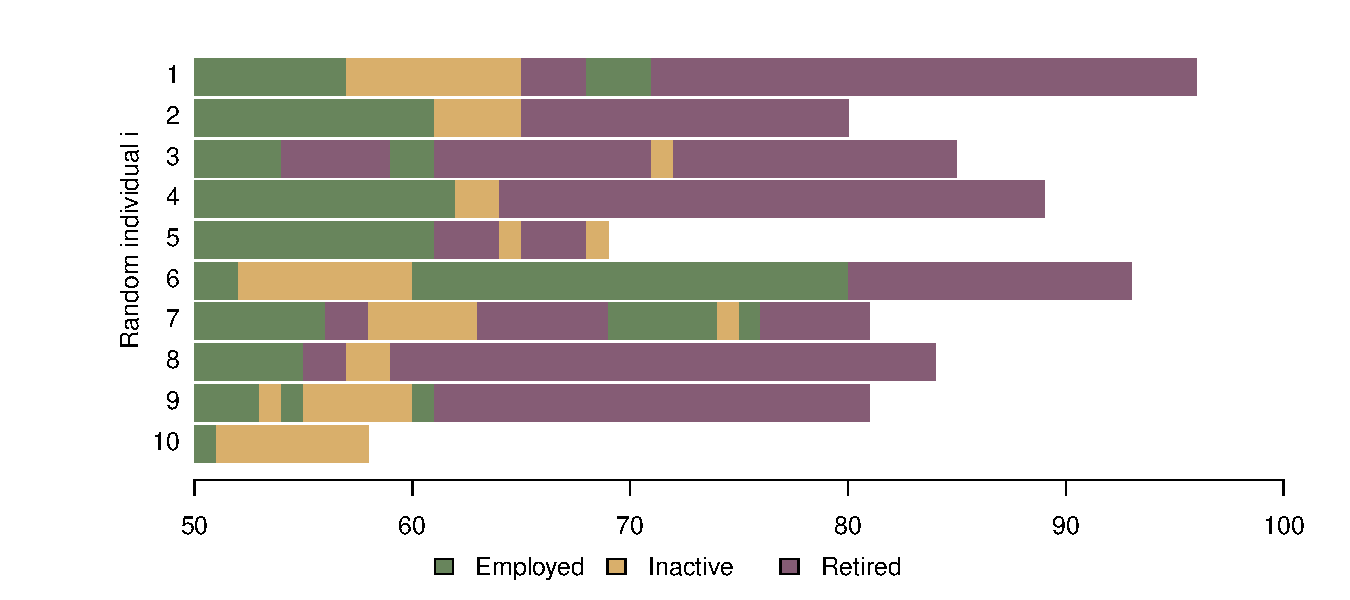
\includegraphics[width=\textwidth, keepaspectratio]{Figures/Seq10.pdf}}
\only<2>{\includegraphics[width=\textwidth, keepaspectratio]{Figures/Seq10clock_prev.pdf}}
\only<3>{\includegraphics[width=\textwidth, keepaspectratio]{Figures/Seq10clock_dur.pdf}}
\only<4>{\includegraphics[width=\textwidth, keepaspectratio]{Figures/Seq10clock_timespent.pdf}}
\only<5>{\includegraphics[width=\textwidth, keepaspectratio]{Figures/Seq10clock_timespentcumul.pdf}}
\only<6>{\includegraphics[width=\textwidth, keepaspectratio]{Figures/Seq10clock_timeleft.pdf}}
\only<7>{\includegraphics[width=\textwidth, keepaspectratio]{Figures/Seq10clock_ordUp.pdf}}
\only<8>{\includegraphics[width=\textwidth, keepaspectratio]{Figures/Seq10clock_ordDown.pdf}}
\end{overlayarea}
\end{center}
\end{frame}

\begin{frame}[plain]
\Large
\begin{center}
\begin{block}{Clock measures}
Measures of scaling or total durations in episodes or cumulatively over episodes; Also
measures of episode order, or even simply prevalence as a simple case.
\end{block}
\pause
Values that get averaged \emph{with respect to some structure}.
\end{center}
\end{frame}

\begin{frame}[plain]
\Large
\begin{center}
Alignment
\vspace{1em}
\begin{overlayarea}{\textwidth}{.4\textheight}
\only<1>{\includegraphics[width=\textwidth, keepaspectratio]{Figures/Seq10aligncoords.pdf}}
\only<2>{\includegraphics[width=\textwidth, keepaspectratio]{Figures/Seq10align_death.pdf}}
\only<3>{\includegraphics[width=\textwidth, keepaspectratio]{Figures/Seq10align_firstret.pdf}}
\only<4>{\includegraphics[width=\textwidth, keepaspectratio]{Figures/Seq10align_longestret.pdf}}
\only<5>{\includegraphics[width=\textwidth, keepaspectratio]{Figures/Seq10align_inactlongleft.pdf}}
\only<6>{\includegraphics[width=\textwidth, keepaspectratio]{Figures/Seq10align_inactlongright.pdf}}
\only<7>{\includegraphics[width=\textwidth, keepaspectratio]{Figures/Seq10align_centerlongempl.pdf}}
%\only<8>{\includegraphics[width=\textwidth, keepaspectratio]{Figures/Seq10clock_ordDown.pdf}}
\end{overlayarea}
\end{center}
\end{frame}

\begin{frame}[plain]
\Large
 \begin{block}{Alignment}
  Shift trajectories to match on a state entry (left) or exit (right) event. The reference event is selected based on a criteria (first, last, longest episode).
 \end{block}
\end{frame}

%
\begin{frame}[plain]
\Large
\begin{center}
\begin{block}{Macro patterns}
Macro patterns can be derived by aggregating (e.g. means) over clock measures by some structure defined by an alignment operation. Clocking and alignment do not need to be with respect to the same state.
\end{block}
\end{center}
\end{frame}
%

\begin{frame}[plain]
\Large
\begin{center}
Inactivity clocks aligned on exit from first retirement
\vspace{2em}
\begin{overlayarea}{\textwidth}{.8\textheight}
\centering
\only<1>{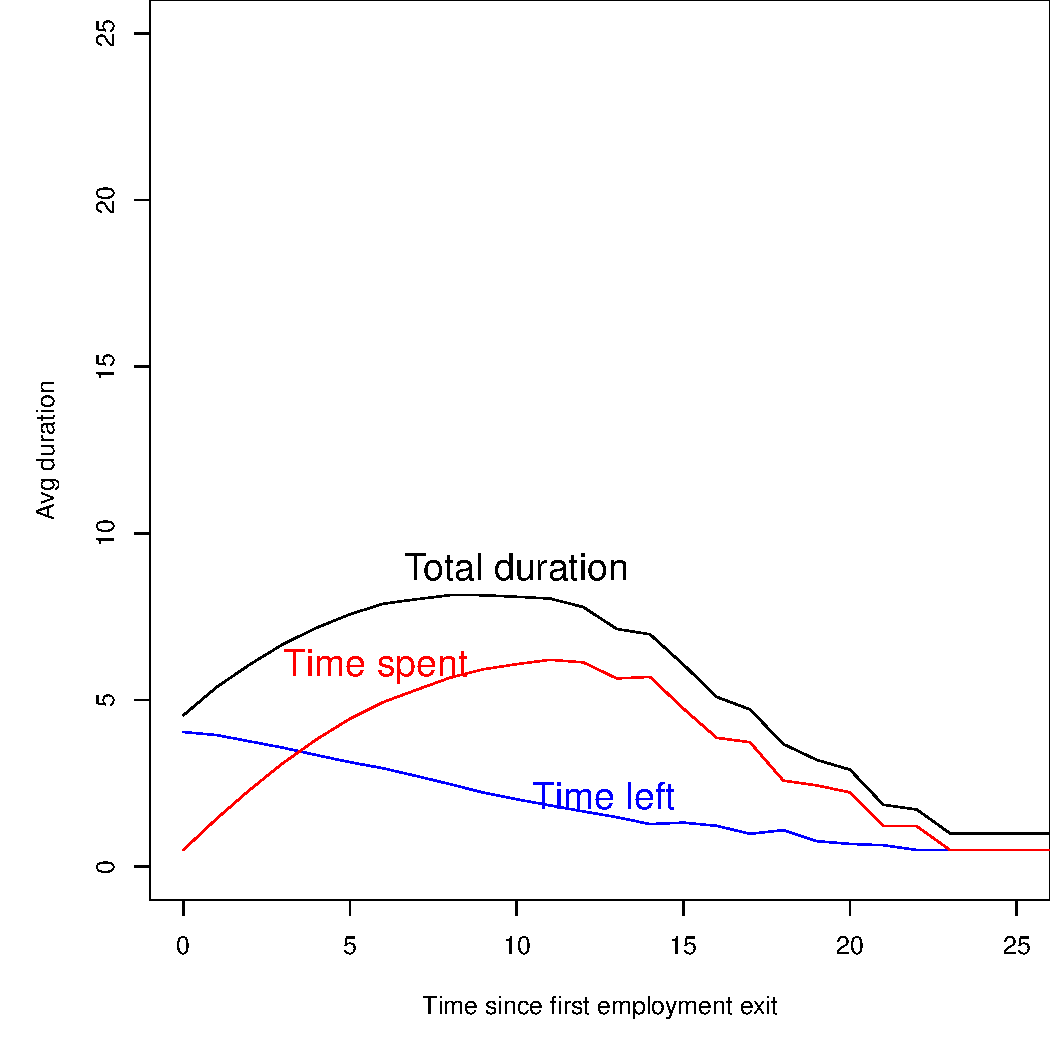
\includegraphics[scale=.9, keepaspectratio]{Figures/Macro1.pdf}}
\only<2>{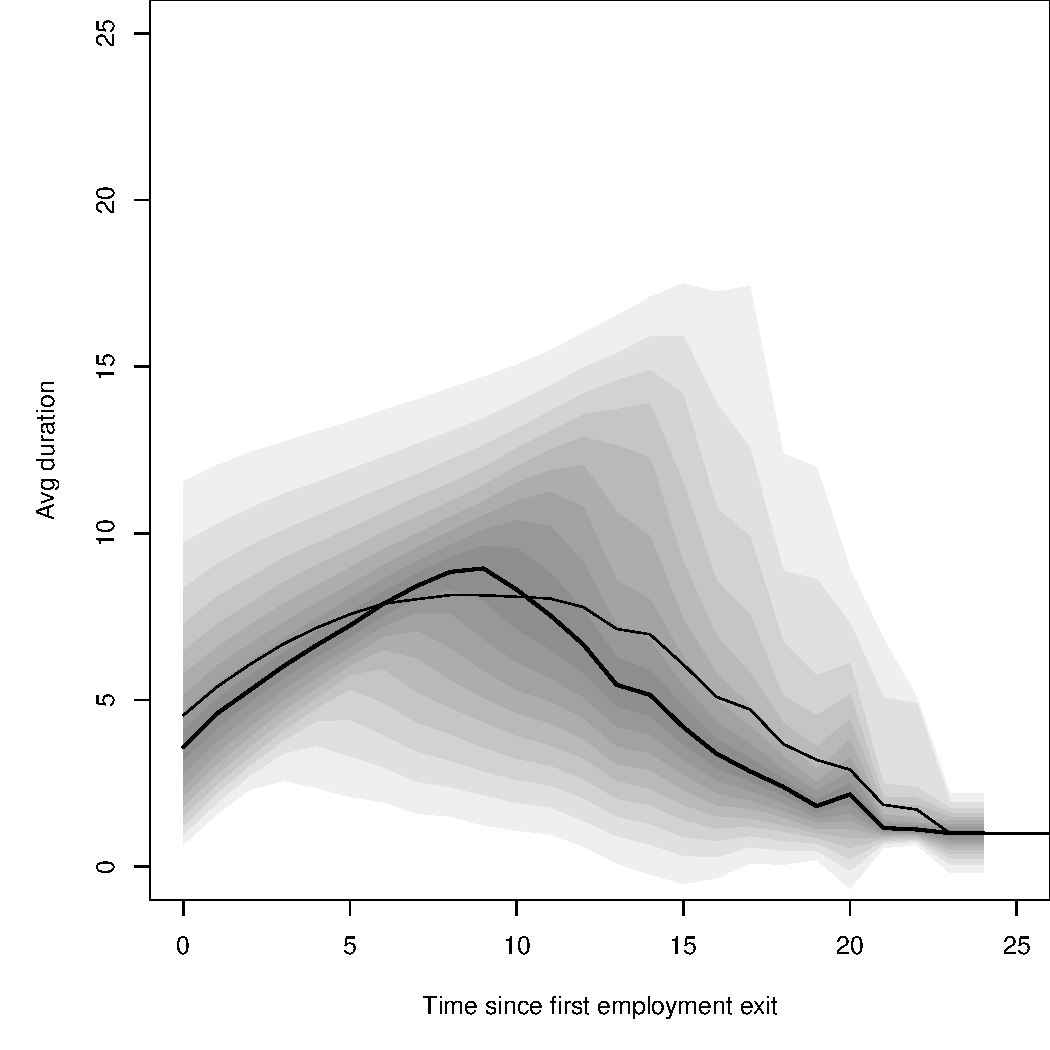
\includegraphics[scale=.9, keepaspectratio]{Figures/Macro2.pdf}}
\only<3>{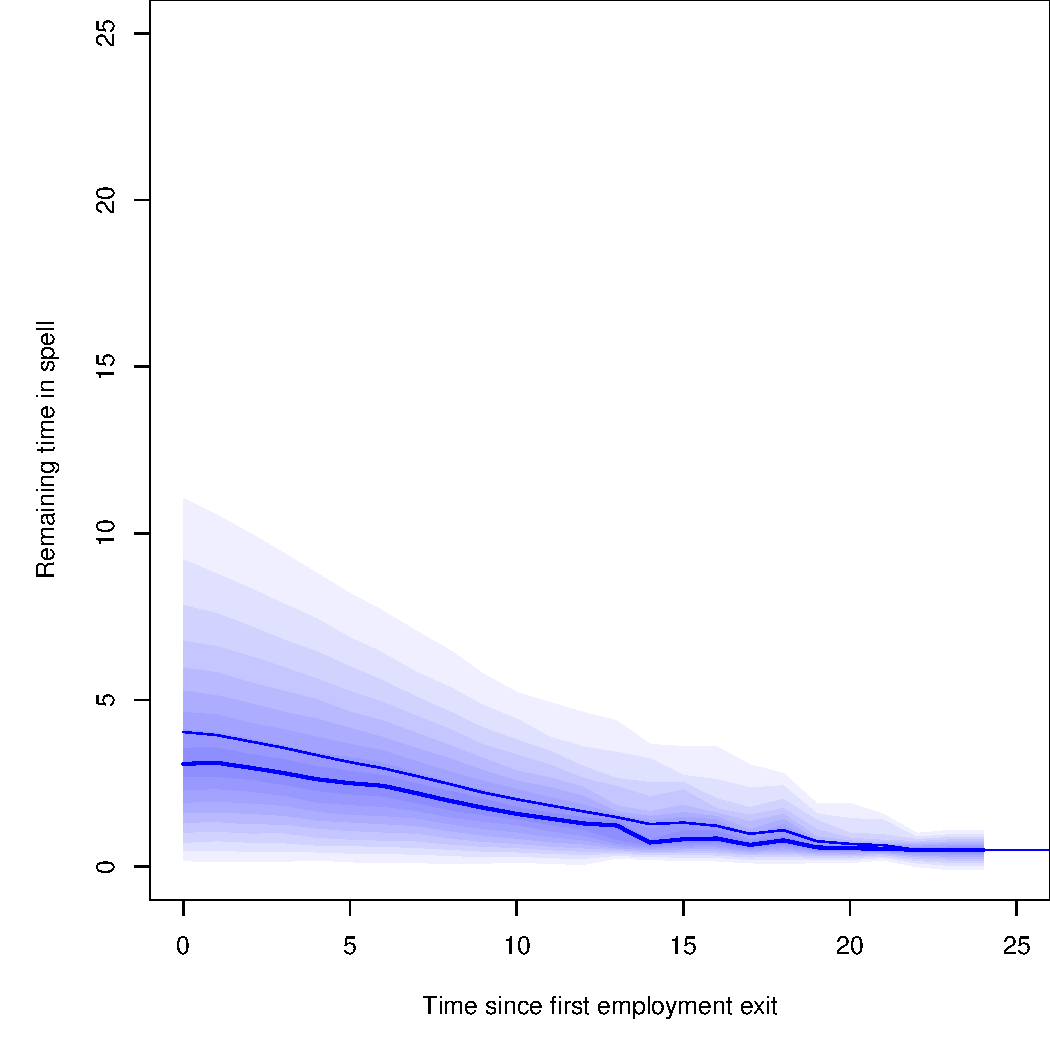
\includegraphics[scale=.9, keepaspectratio]{Figures/Macro3.pdf}}
\only<4>{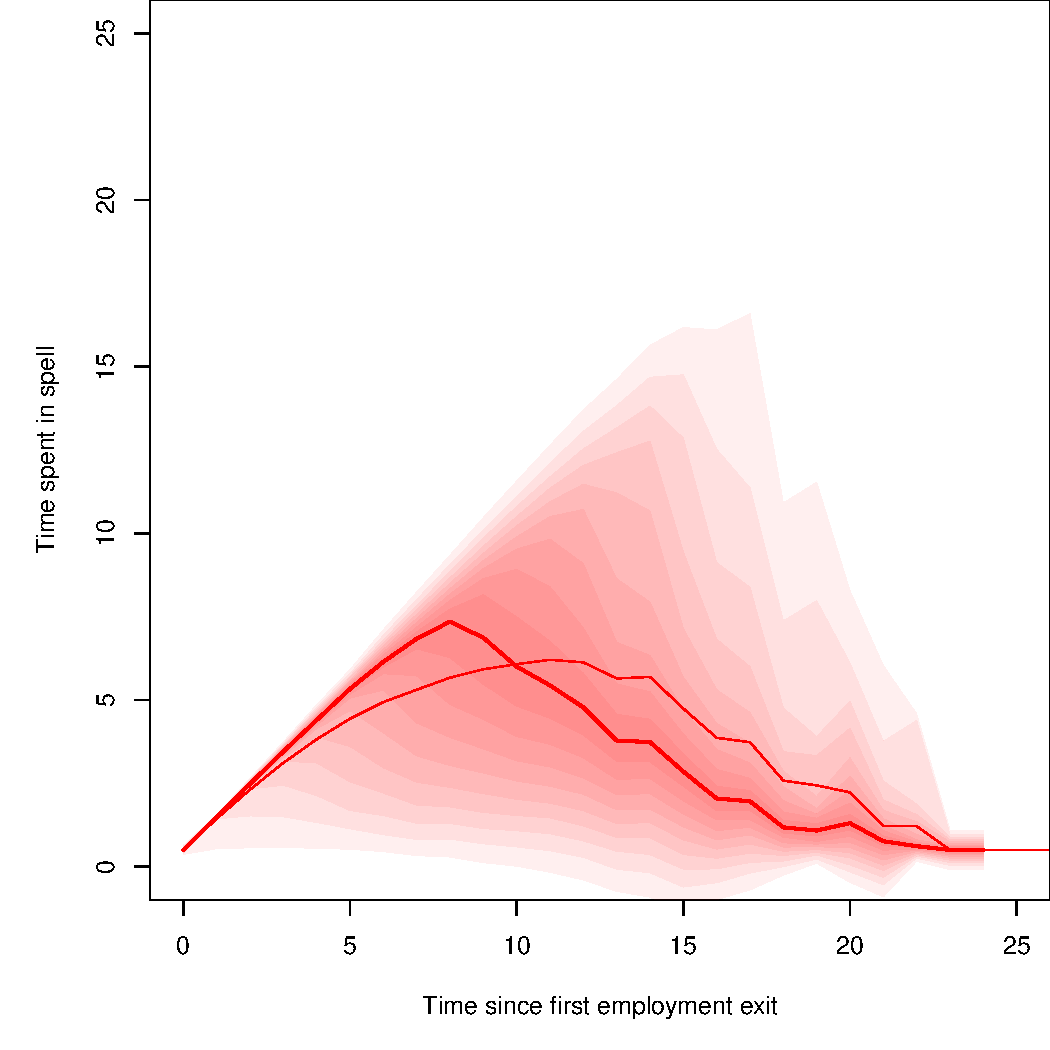
\includegraphics[scale=.9, keepaspectratio]{Figures/Macro4.pdf}}
%\only<8>{\includegraphics[width=\textwidth, keepaspectratio]{Figures/Seq10clock_ordDown.pdf}}
\end{overlayarea}
\end{center}
\end{frame}


\begin{frame}[plain]
\Large
\begin{center}
How many macro patterns from the same data?
\begin{itemize}[<+->]
\item $\textbf{s}$ states
\item $\textbf{a}$ possible alignments (entry, exit, center, \emph{justified}, \ldots)
\item $\textbf{e}$ possible episode choices (first, last, longest episode, \ldots)
\item $\textbf{c}$ possible clock types (up, down, total, order, \emph{fractional}, \emph{relative}, \ldots)
\item $\textbf{s}\times \textbf{a}\times \textbf{e}\times \textbf{c} = \textbf{p}$ possible clock/structure combinations from which to derive macro patterns.
\end{itemize}
\end{center}
\end{frame}
%
\begin{frame}[plain]
\Large
\begin{center}
Why again?
\begin{itemize}[<+->]
\item Preprocessing steps for sequence analyses
\item Pattern detection in general 
\item More completely characterize demographic phenomena 
\item Expand set of possible tenure statistics
\end{itemize}
\pause
Thanks!\\
riffe@demogr.mpg.de
\end{center}


\end{frame}
%



%%%%%%%%%%%%%%%%%%%%%%%%%%%%%%%%%%
%%	End of the document			%%
%%%%%%%%%%%%%%%%%%%%%%%%%%%%%%%%%%
\end{document}






